\section{Experiments}
\newcommand{\msEightyScan}{0.57}
\newcommand{\msEightyBranch}{0.58}
\newcommand{\msEightyKeys}{0.62}
\newcommand{\msNinetyScan}{1.44}
\newcommand{\msNinetyBranch}{1.50}
\newcommand{\msNinetyKeys}{1.74}
\newcommand{\msNinetyFiveScan}{2.87}
\newcommand{\msNinetyFiveBranch}{3.02}
\newcommand{\msNinetyFiveKeys}{3.69}
\newcommand{\msNinetyNineScan}{8.70}
\newcommand{\msNinetyNineBranch}{9.02}
\newcommand{\msNinetyNineKeys}{11.13}
\newcommand{\ratioBoverA}{1.04}
\newcommand{\ratioCoverA}{1.28}
\newcommand{\unitErrorScan}{1.7}
\newcommand{\unitWorstScan}{8}
\newcommand{\unitErrorBranch}{13.7}
\newcommand{\unitWorstBranch}{75}
\newcommand{\unitErrorKeys}{8.0}
\newcommand{\unitWorstKeys}{38}
\newcommand{\scoreMicroseconds}{0.026}
\newcommand{\splitNanoseconds}{0.3}
\newcommand{\lookupNanoseconds}{13}
\newcommand{\settingsMeasured}{189}
\newcommand{\globalScanMs}{26.8}
\newcommand{\globalBranchMs}{745}
\newcommand{\globalBranchSplitWords}{291}
\newcommand{\globalBranchGroups}{36,983}

The experiment has two jobs: check that the code does the work the formulas count, and find
which method is fastest at each recall target. Everything is measured on one machine, an
Apple M5~Max with 128~GiB of RAM, using one CPU thread and one query at a time.

\subsection{Setup}
The inputs are fixed and identical for every setting. The documents are one million
MS~MARCO passages~\cite{msmarco}, embedded with Nomic Embed v1.5~\cite{nomic}, cut to the
first 256 values and stored as 256 sign bits. The 200 queries come from the same collection's
development set. The reference answer for each query is its exact top 100 when all one
million documents are scored. The arrays are read in place; their hashes are recorded before
and after the run and did not change.

What varies is only the index. We use the cluster counts $C\in\{64,256,1024,4096,8192\}$,
with cluster centres learned once by $k$-means~\cite{faiss}, plus the whole collection as a
single cluster. For each $C$, $P$ takes the four values from Table~\ref{tab:routing}, one
per recall target. Every method is measured on all 21 resulting $(C,P)$ pairs, so no
method gets a routing advantage. Within each pair, method A has no further settings; method B
is run without splits, with leaf size 128 and no budget, and with leaf size 128 and node
budgets of 64, 512 and 4,096; method C is run with key widths 4, 8 and 12. That gives
\settingsMeasured\ settings. Each runs in its own process, builds its index from the same
codes, answers the 200 queries twice (once for the slowest setting), and records for every
query the time, the returned IDs and the operation counts of Section~2. We report the median
time over the 400 timings and the mean recall over the 200 queries. The largest process
peak was 1.5~GB, far below the 32~GB limit, so every setting is eligible.

\subsection{Checking the calculations}
Table~\ref{tab:checks} compares the counts that Section~2 predicts from the data and the
settings with the counts the code recorded. Every one matches: the documents scored equal
the documents in the opened clusters, the recall of an exact setting equals the routing
recall $r_{\rm route}$, method B without splits reads exactly $\sum_cW_c$ leaf words, method
C visits all $2^h$ keys and makes $2^hP$ lookups, and the index sizes are the byte counts of
Section~2.2. The work formulas are therefore a correct description of the code.

\begin{table}[htb]\centering\small
\caption{Predicted against recorded counts over the \settingsMeasured\ settings. ``None''
means every setting agreed exactly.}
\label{tab:checks}
\begin{tabular}{@{}lrr@{}}\toprule
Quantity (formula) & Settings checked & Largest difference\\\midrule
Documents scored, $F$ (exact settings) & 126 & 0.00\%\\
Recall $=r_{\rm route}$ (exact settings) & 126 & none\\
Leaf words $V_l$ (B without splits) & 21 & none\\
Split words $V_s$ (B without splits) & 21 & none\\
Keys visited $E=2^h$ & 63 & none\\
Lookups $H=2^hP$ & 63 & none\\
Code bytes $=32N$ & 189 & none\\
ID bytes $=8N$ & 189 & none\\
Bitplane bytes $=8d\sum_cW_c$ & 105 & none\\
Directory bytes $=20U$ & 63 & none\\
\bottomrule\end{tabular}

\end{table}

Turning counts into time needs the constants $c_{\cdot}$. We fit them by least squares on
the measured search times of each method's settings, weighting each setting by its own time
so that fast and slow settings count equally (Table~\ref{tab:units}). Scoring one document
costs about \scoreMicroseconds~$\mu$s in all three methods, a directory lookup about
\lookupNanoseconds~ns, a split word well under a nanosecond, and taking a group from the
queue about a quarter of a microsecond. Figure~\ref{fig:predicted} plots the time the
formula gives against the time measured. For method A the median error is
\unitErrorScan\%, for method C \unitErrorKeys\%, and for method B without splits 11\%.

\begin{table}[htb]\centering\small
\caption{Unit costs from the fit, in microseconds, and the median absolute error of the
fitted formula over each method's settings.}
\label{tab:units}
\begin{tabular}{@{}llrrr@{}}\toprule
Method & Cost & Microseconds & Settings & Median error\\\midrule
A: original & per call, $c_{\rm call}$ & 45.8228 & 21 & 1.7\%\\
 & per scored document, $c_{\rm score}$ & 0.0260 & & \\
B: bitplanes & per call, $c_{\rm call}$ & 9.2597 & 105 & 13.7\%\\
 & per scored document, $c_{\rm score}$ & 0.0295 & & \\
 & per split word, $c_{\rm split}$ & 0.0003 & & \\
 & per leaf word, $c_{\rm leaf}$ & 0.0032 & & \\
 & per group taken from the queue, $c_{\rm group}$ & 0.2394 & & \\
C: backward walk & per call, $c_{\rm call}$ & 11.0438 & 63 & 8.0\%\\
 & per scored document, $c_{\rm score}$ & 0.0308 & & \\
 & per directory lookup, $c_{\rm lookup}$ & 0.0132 & & \\
 & per key generated, $c_{\rm key}$ & 0.0000 & & \\
\bottomrule\end{tabular}

\end{table}

\begin{figure}[htb]\centering
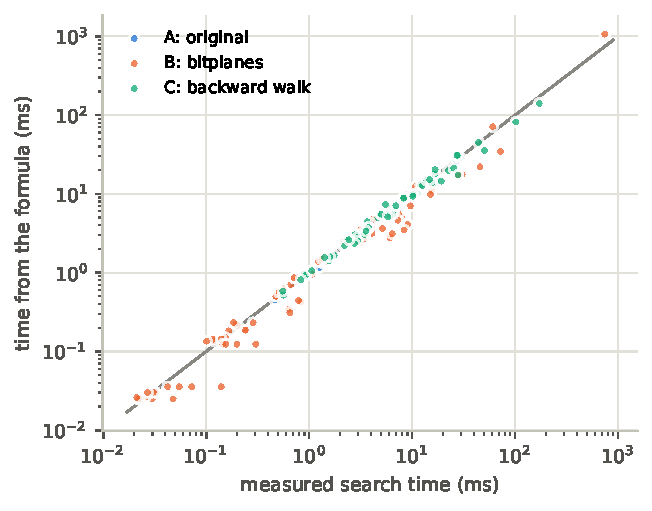
\includegraphics[width=.5\linewidth]{figures/predicted-vs-measured.pdf}
\caption{Search time computed from the recorded counts and the unit costs of
Table~\ref{tab:units}, against the measured median. Points on the grey line are exact.}
\label{fig:predicted}
\end{figure}

The formula is least accurate for method B when it splits wide clusters. At $C=64$ with 37
opened clusters and leaf size 128 the measured time is 72~ms against 35~ms from the formula,
and the single-cluster search with leaf size 128 takes \globalBranchMs~ms against
\globalBranchSplitWords\ million split words and \globalBranchGroups\ groups. The counts
are right; the constants are not constant. When many groups wait in the queue, their masks
and the bitplanes no longer fit in the processor caches, and each word costs several times
more than in the small-cluster settings that dominate the fit. The error runs in one
direction only: splitting is more expensive than the formula says, so it does not change the
comparison below.

\subsection{Results}
Table~\ref{tab:selected} and Figure~\ref{fig:results} give, for each recall target, the
fastest setting of each method that reached the target. Method A is fastest at all four
targets. Method B is behind by 1\% to 4\%, and its fastest setting at every target is the one
without splits, as Section~3.2 derived. Method C is behind by 9\% to 28\% with its narrowest
key, $h=4$, as Section~3.3 derived. All three methods score the same documents at the same
$(C,P)$; the differences are the bookkeeping that Section~3.4 predicted, about
$0.4$~$\mu$s per opened cluster for B and $16$ lookups per opened cluster for C.

\begin{table}[htb]\centering\small
\caption{Fastest setting of each method at each recall target, over all measured settings
that reached the target. Recall is the mean over 200 queries; time is the median per query
including cluster selection.}
\label{tab:selected}
\begin{tabularx}{\linewidth}{@{}llYrrr@{}}\toprule
Target & Method & Setting & Recall & Median ms & Docs scored\\\midrule
80\% & A: original & $C=4,096$, $P=72$ & 80.01\% & 0.569 & 18,107\\
 & B: bitplanes & $C=4,096$, $P=72$; no splits & 80.01\% & 0.576 & 18,107\\
 & C: backward walk & $C=4,096$, $P=72$; $h=4$ & 80.01\% & 0.621 & 18,107\\
\addlinespace[2pt]
90\% & A: original & $C=8,192$, $P=353$ & 90.02\% & 1.442 & 42,847\\
 & B: bitplanes & $C=8,192$, $P=353$; no splits & 90.02\% & 1.496 & 42,847\\
 & C: backward walk & $C=8,192$, $P=353$; $h=4$ & 90.02\% & 1.741 & 42,847\\
\addlinespace[2pt]
95\% & A: original & $C=8,192$, $P=778$ & 95.00\% & 2.872 & 93,930\\
 & B: bitplanes & $C=8,192$, $P=778$; no splits & 95.00\% & 3.022 & 93,930\\
 & C: backward walk & $C=8,192$, $P=778$; $h=4$ & 95.00\% & 3.693 & 93,930\\
\addlinespace[2pt]
99\% & A: original & $C=4,096$, $P=1,330$ & 99.00\% & 8.702 & 325,353\\
 & B: bitplanes & $C=8,192$, $P=2,440$; no splits & 99.00\% & 9.023 & 295,858\\
 & C: backward walk & $C=8,192$, $P=2,440$; $h=4$ & 99.00\% & 11.130 & 295,858\\
\addlinespace[2pt]
\bottomrule\end{tabularx}

\end{table}

\begin{figure}[htb]\centering
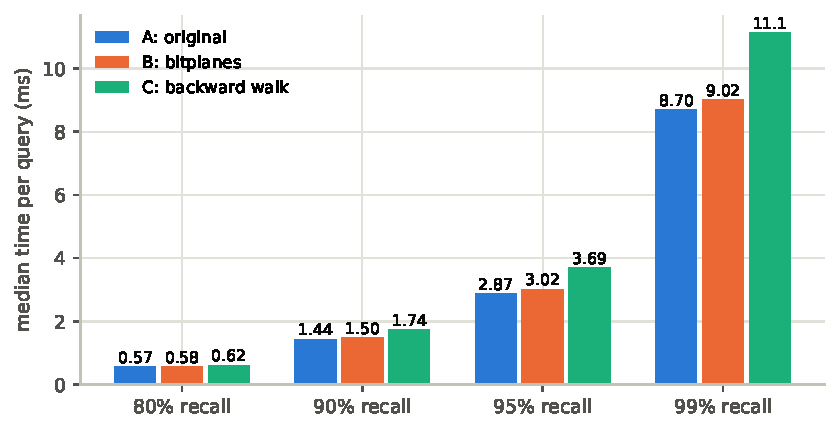
\includegraphics[width=.7\linewidth]{figures/results.pdf}
\caption{The same fastest settings as Table~\ref{tab:selected}. Lower is better.}
\label{fig:results}
\end{figure}

The other settings show the rest of the prediction. For method A, $C=4{,}096$ and
$8{,}192$ are within 1\% of each other at 99\% (8.70 and 8.78~ms), while 64 clusters take
14.9~ms: fewer clusters open more documents, as Table~\ref{tab:routing} says. Cluster
selection itself costs 0.07~ms for 4,096 centres and 0.14~ms for 8,192, growing to 0.37~ms
when 2,440 of them must be sorted out, which is why 4,096 wins at 80\% and 99\% and 8,192
at 90\% and 95\%. For method B, splitting always costs more than it saves: with leaf size
128 and no budget the 99\% setting takes 11.1~ms instead of 9.0, and the 80\% setting
0.79~ms instead of 0.58, because $F_B=F_A$ and the masks are pure overhead. With a budget
the search is faster but loses most of the answer: at $C=8{,}192$, $P=2{,}440$ a budget of
4,096 groups reaches 44\% recall in 5.5~ms and a budget of 512 reaches 37\% in 1.4~ms,
while method A reaches 80\% in 0.57~ms by opening fewer clusters. The best budgeted
setting that reaches 80\% takes 0.72~ms, still behind A. For method C, every extra key bit
doubles the lookups: at the 99\% clusters $h=4$, 8 and 12 take 11.1, 28.3 and 172~ms.
Figure~\ref{fig:all} shows all \settingsMeasured\ settings together.

\begin{figure}[htb]\centering
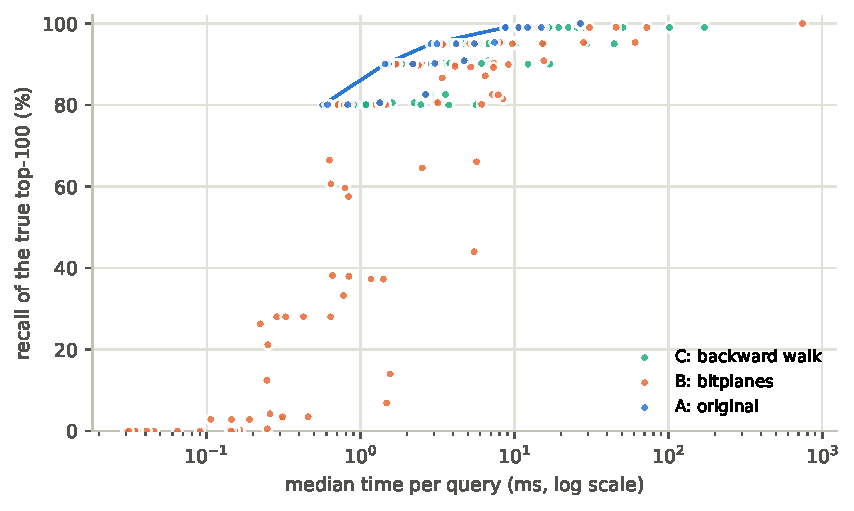
\includegraphics[width=.7\linewidth]{figures/all-settings.pdf}
\caption{Every measured setting. The blue line joins method A's fastest settings at the four
targets. Orange points below 80\% are budgeted bitplane searches; green points beyond 20~ms
are backward walks with wide keys.}
\label{fig:all}
\end{figure}

\subsection{Code references}
The search code is \path{cpp/index.cpp} (method A in \texttt{Index::scan}, method B in
\texttt{Index::search}), \path{cpp/key_index.cpp} (method C) and \path{cpp/score.hpp}
(the shared lookup-table scorer, top-$K$ heap and ceiling rule). The experiment is
\path{experiments/fixed_data_study.py}; each setting is measured by
\path{experiments/worker.py}. The run, with every per-query record, is under
\path{results/fixed-data-2026-09-12/}: \texttt{settings.csv} has one row per setting,
\texttt{selected.csv} the fastest per method and target, \texttt{checks.json} the count
comparisons and \texttt{unit-costs.json} the fit. To repeat the run on this machine:
\begin{lstlisting}
.venv/bin/python -m experiments.fixed_data_study run --output results/my-run
.venv/bin/python reports/search-fixed-data/make_results.py facts
.venv/bin/python reports/search-fixed-data/make_results.py results --run results/my-run
bash reports/search-fixed-data/build.sh
\end{lstlisting}
